\documentclass[11pt]{article}

\usepackage[T1]{fontenc}
\usepackage[english]{babel}

\usepackage{geometry}
\geometry{a4paper, portrait, margin=1.5cm}

\usepackage{xcolor}
\usepackage[most]{tcolorbox}
\usepackage{graphicx}
\usepackage{eso-pic}
\usepackage{setspace}

\usepackage{fontspec} 

\setmainfont[Path = ./fonts/, Ligatures=NoCommon]{Minecraft.ttf} 
\setmonofont[Path = ./fonts/, Ligatures=NoCommon]{Minecraft.ttf}

\renewcommand{\familydefault}{\ttdefault}
\setstretch{1.3} 

\newcommand{\mcheading}[1]{{\fontsize{55}{60}\selectfont #1}}

\newcommand{\mcbody}[1]{{\fontsize{35}{30}\selectfont #1}}

\newcommand{\ctftext}[1]{
  \vspace{1.5em}
  {\raggedright \mcbody{#1}\par}
}

\newcommand{\ctfcmd}[1]{
  \vspace{1.5em}
  {\centering \mcbody{\bfseries #1}\par}
}

\definecolor{mcred}{HTML}{FF5555}  
\definecolor{mcgreen}{HTML}{55FF55}
\definecolor{mcblue}{HTML}{5555FF}
\definecolor{mcgold}{HTML}{FFFF55}
\definecolor{mcdark}{HTML}{1A1A1A}

\pagecolor{white}
\pagestyle{empty}

\begin{document}

\AddToShipoutPictureFG*{%
  \AtPageUpperLeft{%
    \raisebox{-9cm}{%
      \makebox[\paperwidth]{%
        
\includegraphics[width=14cm]{images/logo.png}%
      }%
    }%
  }%
}

\newgeometry{margin=0pt}

\AddToShipoutPictureBG*{%
  \AtPageLowerLeft{%
    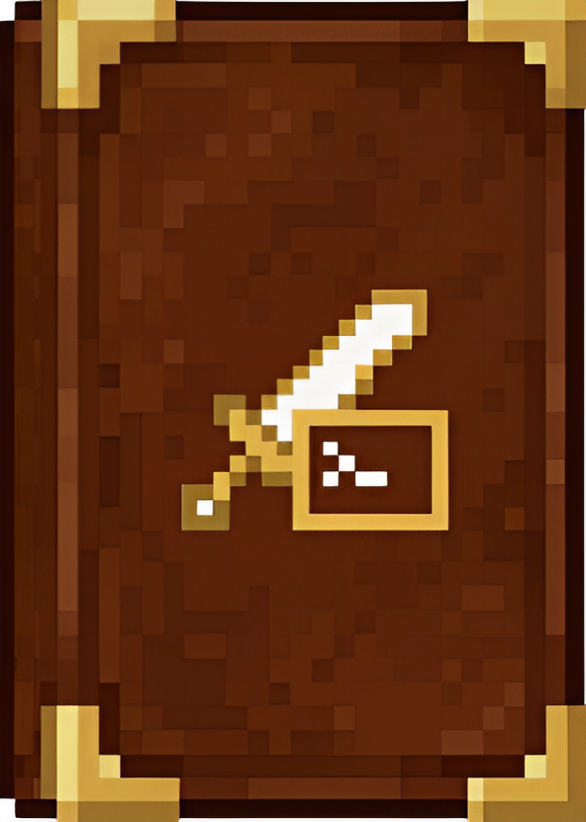
\includegraphics[width=\paperwidth,height=\paperheight]{images/Image.png}%
  }%
}

\begin{minipage}[t][24cm][b]{\paperwidth}
\centering 
\textcolor{white}{
  \mcbody{\textbf{\textit{"Only the one who masters Linux\\ can defeat the Ender Dragon."}}}
}
\end{minipage}

\newpage

\ClearShipoutPictureFG

\restoregeometry

\AddToShipoutPictureBG{%
  \AtPageLowerLeft{%
    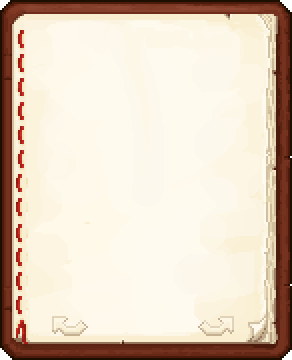
\includegraphics[width=\paperwidth,height=\paperheight]{images/background.png}%
  }%
}

\centering 
\begin{minipage}{0.85\textwidth} 
\textcolor{white}{ 

\vspace{5em}
\textcolor{mcred}{\mcheading{\bfseries 1. Overworld Discover}}

\ctftext{The world generates events in real-time. Open a second terminal and monitor the global server log to keep track of changes:}
\ctfcmd{tail -f /var/log/ \\ minecraft\_server.log}

\ctftext{Mineshafts hold many secrets. Map out hidden structures inside the project directory and filter out empty decoy files:}
\ctfcmd{ls -la}
\ctfcmd{find . -type f -size +0c}

\vspace{5em}
\textcolor{mcred}{\mcheading{\bfseries 1. Loot Analysis}}

\ctftext{Your scan has revealed hidden assets across the shafts. Here is what they truly represent:}
\end{minipage}

\newpage
\centering 
\begin{minipage}{0.85\textwidth} 
\textcolor{white}{ 
\vspace{4em}

\ctftext{1. .hidden\_crevice/golden\_apple.txt - A golden apple artifact hiding your first secret flag. Read it:}
\ctfcmd{cat east-shaft/.hidden\_crevice/ \\ golden\_apple.txt}

\ctftext{2. .lost\_library/secret\_room/ \\ book\_of\_wisdom.py - An ancient book of the old sage. Put it in your universal inventory (the /tmp directory) to carry it across dimensions and decode runes later:}
\ctfcmd{cp .lost\_library/secret\_room/ \\ book\_of\_wisdom.py /tmp/}

\ctftext{3. north\_shaft/flooded\_section/ \\ mysterious\_gem.png - A raw gem resource disguised with a fake extension. Inspect its type:}
\ctfcmd{file north-shaft/flooded\_section/ \\ mysterious\_gem.png}

\ctftext{It is actually a pure text file! Read its core content to claim your second hidden flag:}
\ctfcmd{cat north-shaft/flooded\_section/ \\ mysterious\_gem.png}

\end{minipage}

\newpage

\centering 
\begin{minipage}{0.85\textwidth} 
\textcolor{white}{ 

\vspace{5em}

\textcolor{mcblue}{\mcheading{\bfseries 2. Archive Search}}

\ctftext{Now find your path to the Nether. Breach the secret library room and analyze the massive server logs to filter out noisy messages and find administrative errors:}
\ctfcmd{grep "ERROR" .lost\_library/ \\ server\_logs.txt}

\ctftext{The logs mention an old world backup stored away in the dark. Locate the compressed archive file inside the old mineshaft and extract it:}
\ctfcmd{tar -xzf world\_backup\_2011.tar.gz}

\AddToShipoutPictureFG*{%
  \AtPageUpperLeft{%
    \raisebox{-26cm}{%
      \makebox[\paperwidth]{%
        
\includegraphics[width=7cm]{images/table.png}%
      }%
    }%
  }%
}
}
\end{minipage}

\newpage

\centering 
\begin{minipage}{0.85\textwidth} 
\textcolor{white}{  

\vspace{5em}

\textcolor{mcblue}{\mcheading{\bfseries 2. Ancient Diary}}

\ctftext{The world backup archive is now successfully unpacked. Navigate into the temporary folder and extract the final records from the recovered miner's diary:}
\ctfcmd{cat world\_backup/ \\ miners\_diary.txt}

\AddToShipoutPictureFG*{%
  \AtPageUpperLeft{%
    \raisebox{-24cm}{%
      \makebox[\paperwidth]{%
        
\includegraphics[width=8cm]{images/diary.png}%
      }%
    }%
  }%
}
}
\end{minipage}

\newpage

\centering
\begin{minipage}{0.85\textwidth}
\textcolor{white}{

\vspace{5em}

\textcolor{mcred}{\mcheading{\bfseries 3. Light the Way}}

\ctftext{Locate the pitch black secret mine path. You cannot see anything here. Craft a working torch by writing the active power keyword into the file:}
\ctfcmd{echo "light" > .abandoned\_mineshaft/ \\ .deep\_cave/.secret\_mine/torch.txt}

\ctftext{The flame wakes up a guard! A dangerous zombie process spawns instantly to protect the cache. Delete its file to terminate the threat:}
\ctfcmd{rm .abandoned\_mineshaft/.deep\_cave/ \\ .secret\_mine/zombie.txt}

\ctftext{The monster drops a chest on the ground. Read the parchment inside to uncover credentials for the next dimensions:}
\ctfcmd{cat .abandoned\_mineshaft/.deep\_cave/ \\ .secret\_mine/chest.txt}
}
\end{minipage}

\newpage

\centering
\begin{minipage}{0.85\textwidth}
\textcolor{white}{

\vspace{5em}

\textcolor{mcblue}{\mcheading{\bfseries 4. Nether Stash}}

\ctftext{Cross the dimensional border. Use your credentials to log in as the nether traveler session user:}
\ctfcmd{su nether\_traveler \\ \vspace{0.5em} Password: MinecraftCTF\{portal\_ignited\}}

\ctftext{Track the footprints of the previous traveler. Inspect the shell environment execution history log to leak their emergency stash code:}
\ctfcmd{cat \string~/.bash\_history}

\AddToShipoutPictureFG*{%
  \AtPageUpperLeft{%
    \raisebox{-25cm}{%
      \makebox[\paperwidth]{%
        
\includegraphics[width=7cm]{images/star.png}%
      }%
    }%
  }%
}
}
\end{minipage}

\newpage

\centering
\begin{minipage}{0.85\textwidth}
\textcolor{white}{

\vspace{5em}

\textcolor{mcred}{\mcheading{\bfseries 5. Enchanting}}

\ctftext{Go to the nether folder and inspect the ancient text on the enchanting table. It holds three base64 runtime ciphers:}
\ctfcmd{cat nether/enchanting\_table.txt}

\ctftext{Use the book of wisdom Python script from your universal inventory to pass and decode the true name of the Sharpness V rune:}
\ctfcmd{python3 /tmp/book\_of\_wisdom.py \\ "U2hhcnBuZXNzIFY="}

\ctftext{Cast the spell by writing the decoded enchantment directly into your combat file setup:}
\ctfcmd{echo "Sharpness V" > nether/ \\ enchanted\_sword.txt}
}
\end{minipage}

\newpage

\centering
\begin{minipage}{0.85\textwidth}
\textcolor{white}{

\vspace{5em}

\textcolor{mcblue}{\mcheading{\bfseries 6. Wither Battle}}

\ctftext{Before you advance, complete the altar ritual. Move the skull item file into the active altar directory to open the gates:}
\ctfcmd{mv nether/wither\_skull.txt \\ nether/altar\_of\_fire/}

\ctftext{Enter the fortress zone. The boss has a 000 file system shield. Break its immunity settings and destroy it completely:}
\ctfcmd{cd nether/wither\_fortress/ \\  chmod 777 wither\_boss.txt \\ \vspace{1em} rm wither\_boss.txt}

\AddToShipoutPictureFG*{%
  \AtPageUpperLeft{%
    \raisebox{-27cm}{%
      \makebox[\paperwidth]{%
        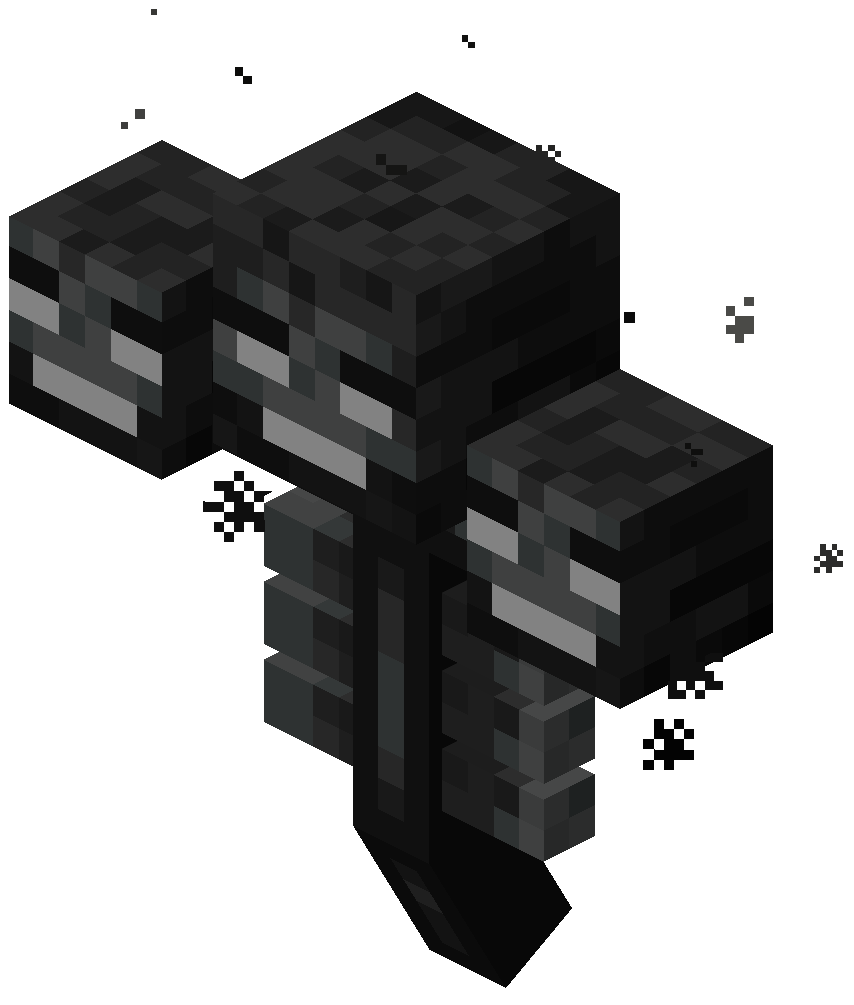
\includegraphics[width=6cm]{images/Wither.png}%
      }%
    }%
  }%
}

\end{minipage}

\newpage

\centering
\begin{minipage}{0.85\textwidth}
\textcolor{white}{

\vspace{5em}

\textcolor{mcred}{\mcheading{\bfseries 7. The End Portal}}

\ctftext{Collect the nether star drop file. Now establish a secure remote network shell tunnel to jump straight into the end dimension framework:}
\ctfcmd{ssh ender\_traveler@localhost \\ \vspace{0.5em} Password: \\ MinecraftCTF\{dragon\_slayer\}}

\ctftext{The portal path is silent. Schedule your arrival time at 12:00 in the user cron table to trigger the portal event. Add this exact line at the bottom of the file:}
\ctfcmd{crontab -e \\ \vspace{0.5em} 0 12 * * * /bin/true}

\ctftext{The dragon is protected by a background service. Locate the systemd daemon and stop it completely:}
\ctfcmd{systemctl stop \\ ctf-spawner.service}

\end{minipage}

\newpage

\centering
\begin{minipage}{0.85\textwidth}
\textcolor{white}{ 

\vspace{5em}

\textcolor{mcblue}{\mcheading{\bfseries 8. Freeing the End}}

\ctftext{With the spawners down, you must now slay the remaining protective endermen guards. Use a wildcard to purge all text entities, then destroy the main core dragon directory tree to finish the run:}
\ctfcmd{rm the\_end/*.txt \\ \vspace{0.5em} rm -rf the\_end/ender\_dragon}

\vspace{3em}

\begin{center}
\mcheading{\textcolor{mcgreen}{\bfseries MinecraftCTF\{}}\\
\vspace{0.3em}
\mcheading{\textcolor{mcgreen}{\bfseries ultimate\_linux\_master\}}}
\end{center}

\AddToShipoutPictureFG*{%
  \AtPageUpperLeft{%
    \raisebox{-23cm}{
      \makebox[\paperwidth]{
        
\includegraphics[width=11cm]{images/theend.png}
      }
    }
  }%
}
\end{minipage}
\end{document}
